\documentclass[a4paper,12pt]{article}

% Configuração de idioma e codificação
\usepackage[utf8]{inputenc}
\usepackage[T1]{fontenc}
\usepackage[brazil]{babel}

% Layout da página
\usepackage[a4paper, margin=0.8in]{geometry}
\usepackage{setspace}
\setstretch{1.5} % Espaçamento entre linhas

% Fontes e formatação
\usepackage{kpfonts}
\usepackage{amsmath, bm} % Pacotes matemáticos
\usepackage{graphicx} % Inclusão de imagens
\usepackage{caption} % Estilização de legendas
\usepackage{fancyhdr} % Personalização de cabeçalhos e rodapés
\usepackage{titlesec} % Personalização de títulos de seção
\usepackage{xcolor} % Cores para textos e seções
\usepackage{hyperref} % Links clicáveis
\usepackage{background} % Fundo para a página de título
\usepackage{placeins} % Controle de posicionamento de floats (FloatBarrier)
\usepackage{pdfpages}
% Ensure the package is loaded correctly for \floatbarrier

\hypersetup{
    colorlinks=true,
    linkcolor=red,
    urlcolor=red,
    citecolor=red
}

% Personalização dos títulos
\titleformat{\section}{\Large\bfseries\color{black}}{\thesection}{1em}{}
\titleformat{\subsection}{\large\bfseries\color{black}}{\thesubsection}{1em}{}

% Cabeçalhos e Rodapés
\pagestyle{fancy}
\fancyhf{}
\fancyhead[R]{
\includegraphics[width=2cm]{ITA.png}} % Logo no topo direito
\fancyhead[L]{\textbf{Instituto Tecnológico de Aeronáutica (ITA)}}
\fancyfoot[L]{Leonardo Peres Dias}
\fancyfoot[R]{\thepage}

% Informações do título
\title{
    \textbf{Inteligência Artificial para Robótica Móvel CT-213}\\
    \Large Instituto Tecnológico de Aeronáutica 

    \textbf{Relatório do Laboratório 9 - Detecção de Objetos}\\
}
\author{
    Leonardo Peres Dias 
}
\date{\today}

% Configuração do fundo (marca d'água apenas na primeira página)
\backgroundsetup{
    scale=1.5,
    color=black,
    opacity=0.2,
    angle=0,
    position=current page.south,
    vshift=5cm,
    hshift=0cm,
    contents={
\includegraphics[width=8cm]{ITA.png}}
}

% Início do Documento
\begin{document}

% Aplicar o fundo apenas na primeira página
\BgThispage
\maketitle
\thispagestyle{empty} % Sem cabeçalho/rodapé na página de título

%\begin{abstract}
%Este documento apresenta o relatório do Projeto CES-30 - 2024, desenvolvido com base na segunda forma descrita no enunciado do exame. O projeto abrange tarefas de \textbf{mineração de dados} e \textbf{construção de grafos de conhecimento}, com a aplicação de técnicas específicas para análise e solução prática de problemas reais.
%\end{abstract}

\newpage
\NoBgThispage % Desativa a marca d'água para as páginas seguintes

\tableofcontents

\newpage
\NoBgThispage % Desativa a marca d'água para as páginas seguintes

\section{Breve Explicação em Alto Nível da Implementação}

A rede neural convolucional implementada para detecção de objetos segue uma arquitetura inspirada no modelo YOLO (You Only Look Once), adaptada para imagens com resolução de $120 \times 160$ pixels. A saída da rede possui dimensões $(15, 20, 10)$, correspondendo a uma grade de $15 \times 20$ células, cada uma com um vetor de 10 atributos.

A arquitetura é composta por nove camadas convolucionais principais, intercaladas com \textit{Batch Normalization} e funções de ativação Leaky ReLU. O modelo pode ser dividido em três blocos principais:

\begin{itemize}
    \item \textbf{Extração de características}: As primeiras camadas convolucionais extraem características locais da imagem, com aumento progressivo da profundidade do mapa de ativação (de 8 até 64 filtros), seguidas por operações de \textit{MaxPooling} que reduzem a resolução espacial.

    \item \textbf{Bloco de salto (skip connection)}: Após a sexta camada convolucional, é realizada uma conexão residual, permitindo o reaproveitamento de características de nível intermediário.

    \item \textbf{Concatenação e previsão}: As saídas da skip connection e da oitava camada convolucional são concatenadas. Em seguida, uma última convolução $1 \times 1$ com 10 filtros gera a saída final, representando as probabilidades e parâmetros das bounding boxes para bola e traves.
\end{itemize}

Já a classe \texttt{YoloDetector} implementa a lógica de detecção de objetos (bola e traves) a partir de imagens da câmera do robô, utilizando uma rede neural do tipo YOLO treinada previamente e salva no formato \texttt{.hdf5}.

\begin{itemize}
    \item \textbf{Inicialização do modelo}: no método \texttt{\_\_init\_\_()}, o modelo é carregado com a função \texttt{load\_model} do Keras e os tamanhos das \textit{anchor boxes} para bola e trave são definidos.

    \item \textbf{Pré-processamento da imagem}: o método \texttt{preprocess\_image()} redimensiona a imagem de entrada de $640 \times 480$ para $160 \times 120$ e normaliza os pixels para o intervalo $[0, 1]$. O formato final da imagem se torna $(1, 120, 160, 3)$, compatível com a entrada da rede.

    \item \textbf{Inferência e detecção}: o método \texttt{detect()} realiza a predição da rede neural com a imagem processada e chama \texttt{process\_yolo\_output()} para extrair as detecções.

    \item \textbf{Processamento da saída da rede}: o método \texttt{process\_yolo\_output()} interpreta a saída da rede YOLO, que possui formato $(15, 20, 10)$. Cada célula da grade representa uma sub-região da imagem e contém:

    \begin{itemize}
        \item Para a bola: $(t_b, t_{xb}, t_{yb}, t_{wb}, t_{hb})$
        \item Para as traves: $(t_p, t_{xp}, t_{yp}, t_{wp}, t_{hp})$
    \end{itemize}

    Os valores $t$ são transformados, sendo posteriormente multiplicados por fatores de escala e pelas dimensões das \textit{anchor boxes}. A célula com maior probabilidade para a bola é selecionada, e as duas melhores para as traves são escolhidas.

    \item \textbf{Formato final da detecção}: cada objeto detectado é representado por uma tupla de 5 elementos: $(\text{probabilidade}, x, y, \text{largura}, \text{altura})$, indicando a confiança da detecção e a caixa delimitadora no espaço da imagem original.
\end{itemize}

\newpage

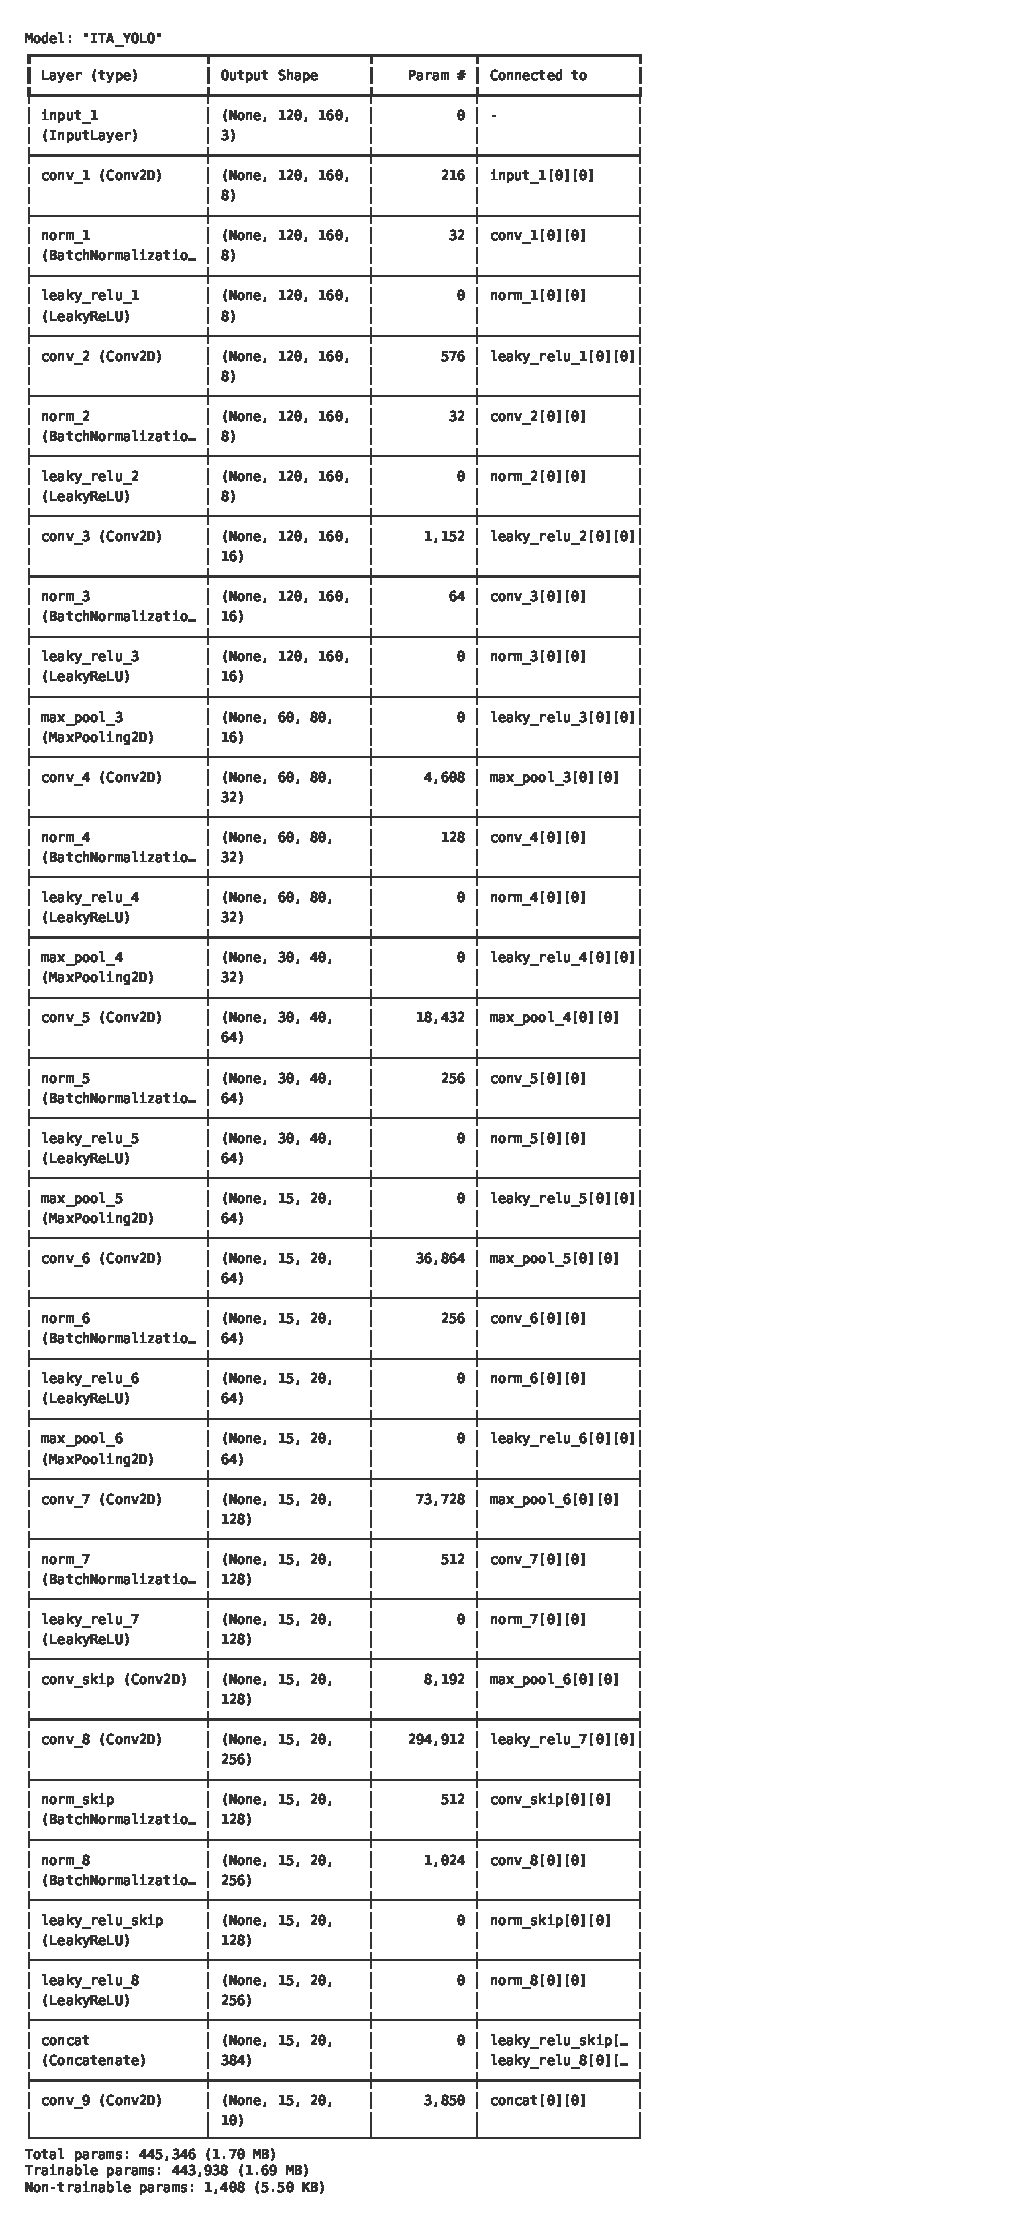
\includepdf[pages=-, pagecommand={}, scale=0.90]{ITA_YOLO_model_summary_COMPLETE.pdf}

\newpage

\section{Figuras Comprovando Funcionamento do Código}

\begin{figure}[htbp]
    \centering
    % Primeira linha: três imagens
    \begin{minipage}[b]{0.3\textwidth}
        \centering
        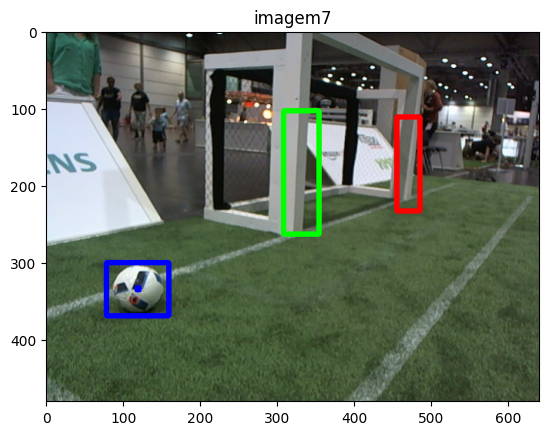
\includegraphics[width=\textwidth]{imagem1.png}
        
    \end{minipage}
    \hfill
    \begin{minipage}[b]{0.3\textwidth}
        \centering
        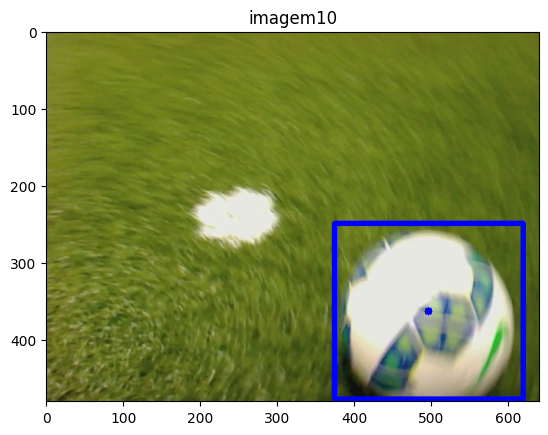
\includegraphics[width=\textwidth]{imagem2.png}
      
    \end{minipage}
    \hfill
    \begin{minipage}[b]{0.3\textwidth}
        \centering
        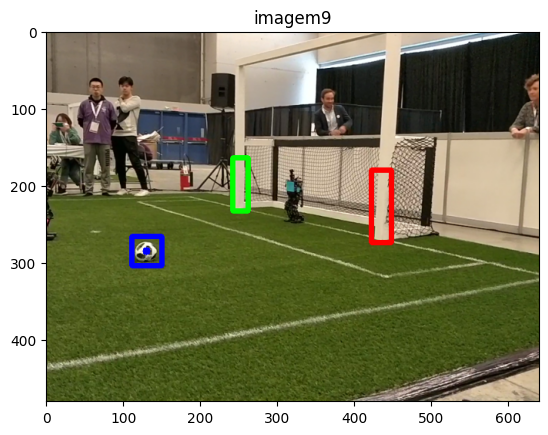
\includegraphics[width=\textwidth]{imagem3.png}
 
    \end{minipage}
    
    \vspace{0.5cm}
    
    % Segunda linha: duas imagens centralizadas
    \begin{minipage}[b]{0.45\textwidth}
        \centering
        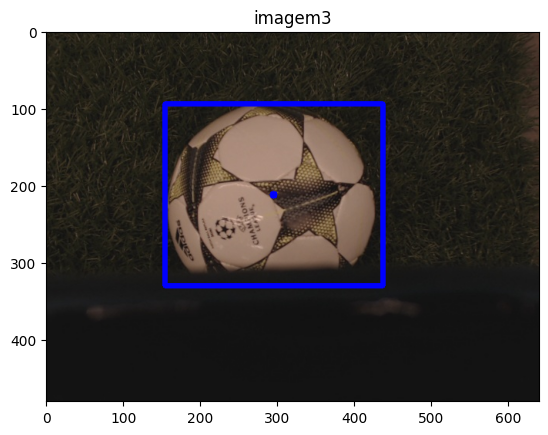
\includegraphics[width=\textwidth]{imagem4.png}

    \end{minipage}
    \hfill
    \begin{minipage}[b]{0.45\textwidth}
        \centering
        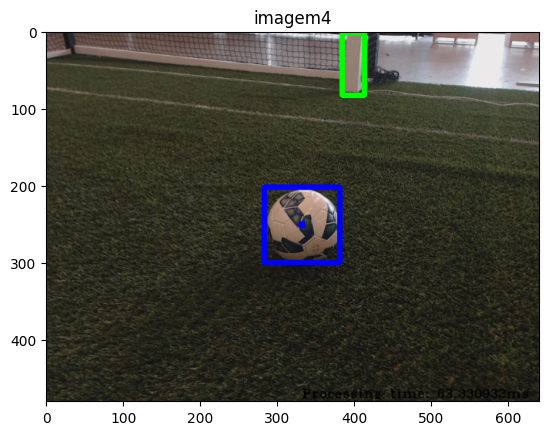
\includegraphics[width=\textwidth]{imagem5.png}
   
    \end{minipage}
    \caption{Exemplos de deteção feitas pela YOLO.}
\end{figure}

\section{Discussão}

As figuras mostram que o detector é capaz de localizar corretamente a bola (caixa azul) e as traves (caixas verde e vermelha) em diferentes cenários. A bola foi detectada com precisão em diversas escalas e posições, mesmo quando parcialmente ocluída. As traves também foram bem identificadas, inclusive em imagens com perspectiva ou múltiplos elementos no fundo. Os resultados indicam que a rede generaliza bem para diferentes situações do jogo.

\end{document}